\subsection{External validation with unused tables}
The frozen $k=2$ labels were checked against tables that never entered clustering: household demographics (801 households) and campaign/coupon records. Labels are not refit. H and L denote the higher- and lower-activity groups within a space (higher mean calibration spend; RFM cluster 1, Product cluster 0). All associations are observational.

\paragraph{Demographics.} Coverage is extremely uneven (Figure~\ref{fig:demographics}). Demographics exist for 773 of 1,616 RFM-H households (47.8\%) but only 28 of 882 RFM-L households (3.2\%); for Product, 766 of 1,655 (46.3\%) versus 35 of 843 (4.2\%) (coverage difference $p<10^{-100}$ in both spaces). The demographic sample is therefore almost entirely a higher-activity sample, the L comparison rests on 28--35 households, and nothing here describes low-activity households in general. Table~\ref{tab:demotests} shows no demographic variable differs significantly between groups at the 5\% level, with small effect sizes (Cram\'er's $V\leq0.11$); no result survives Holm correction. Several cells have expected counts below five, so the chi-square approximations are rough, and the tests have little power. Descriptively, L households show a larger share of 5+ person households and of households with three or more children in both spaces, but these patterns are not statistically supported. Income bands above \$100K were merged for testing.
\begin{table}[htbp]\centering\small
\caption{Chi-square tests of independence between frozen group and demographic variable (households with demographics only). $V$ is Cram\'er's $V$.}\label{tab:demotests}
\begin{tabular}{lrrrrrr}\toprule
 & \multicolumn{3}{c}{RFM} & \multicolumn{3}{c}{Product}\\\cmidrule(lr){2-4}\cmidrule(lr){5-7}
Variable & $\chi^2$ & $p$ & $V$ & $\chi^2$ & $p$ & $V$\\\midrule
Age & 5.82 & 0.324 & 0.09 & 1.74 & 0.884 & 0.05\\
Income & 9.54 & 0.089 & 0.11 & 6.08 & 0.299 & 0.09\\
Household size & 4.76 & 0.313 & 0.08 & 9.15 & 0.057 & 0.11\\
Kids & 5.02 & 0.171 & 0.08 & 6.13 & 0.105 & 0.09\\
Homeowner & 1.45 & 0.835 & 0.04 & 1.64 & 0.802 & 0.05\\\bottomrule
\end{tabular}
\end{table}
\begin{figure}[htbp]\centering
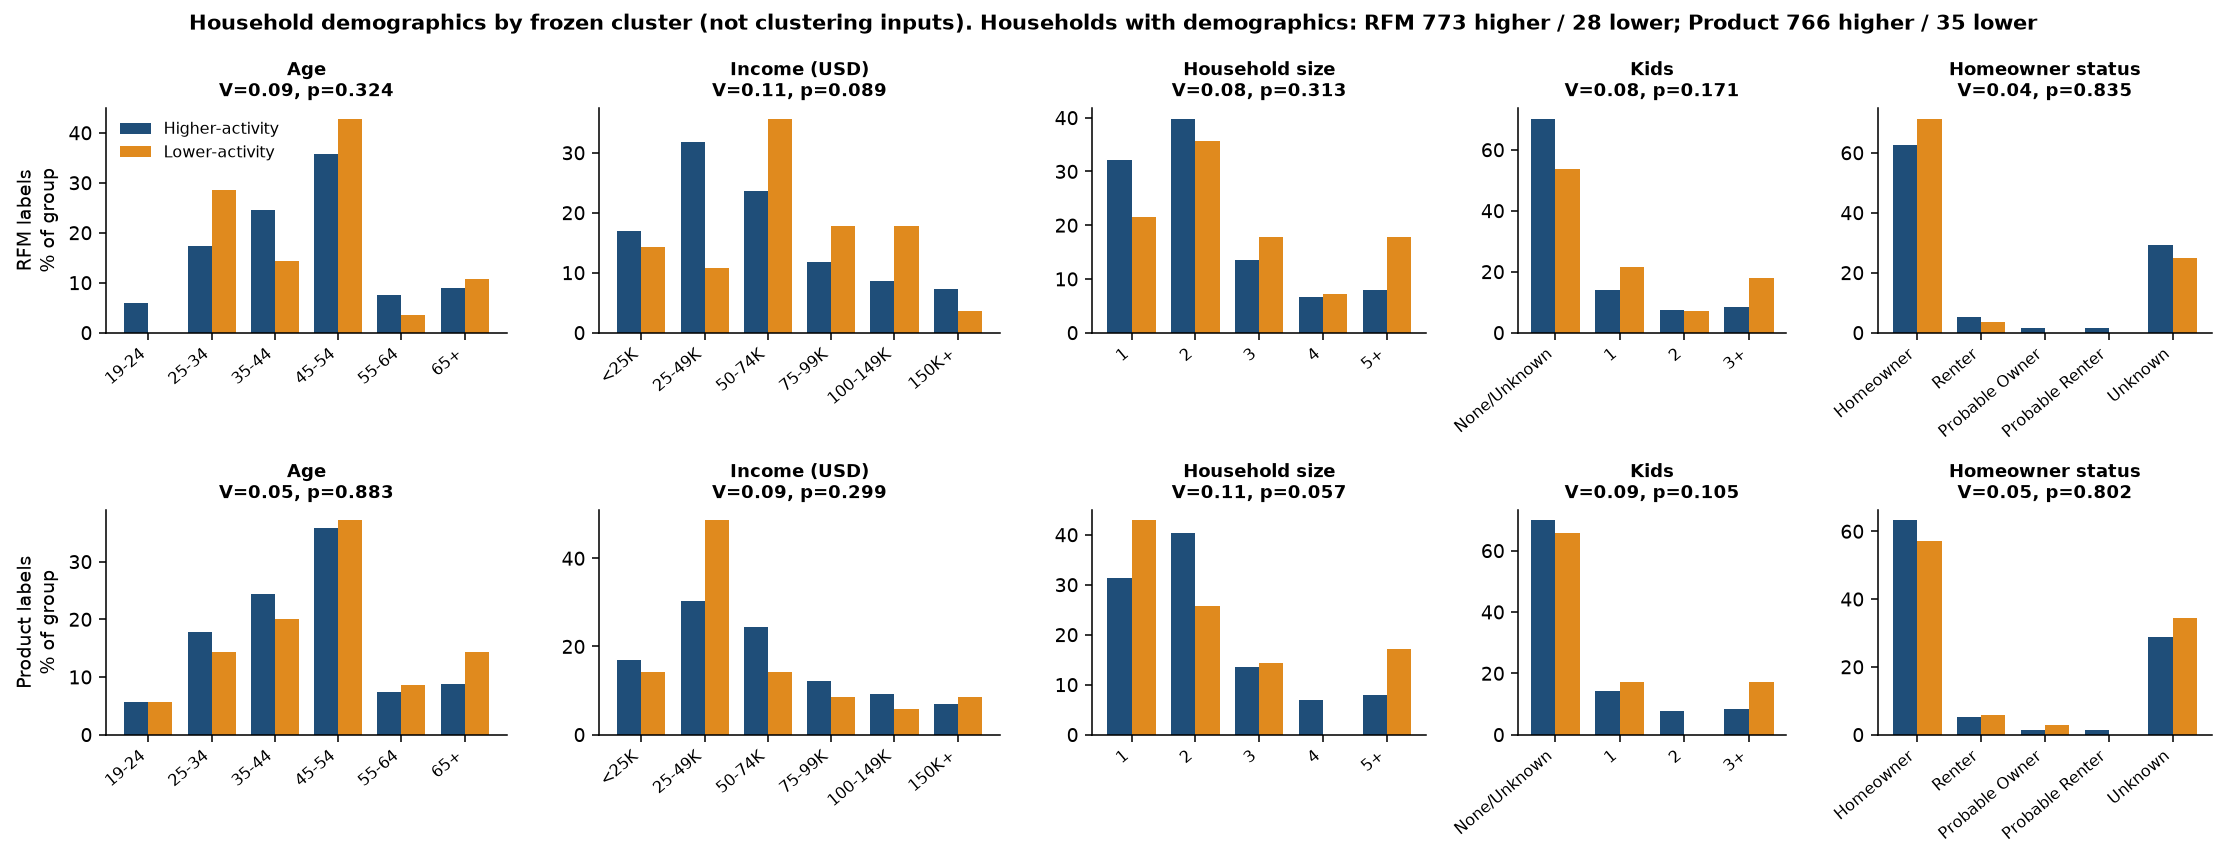
\includegraphics[width=\textwidth]{../figures/14_demographics.png}
\caption{Demographic distributions by frozen group. Panel titles report $V$ and the chi-square $p$ value. The L bars rest on only 28 (RFM) or 35 (Product) households.}\label{fig:demographics}
\end{figure}

\paragraph{Campaign and coupon response.} Only campaigns starting after day 500 are used (campaigns 13--25), so targeting and response are out-of-sample relative to the calibration features. A household is \emph{targeted} if it appears in \texttt{campaign\_table} for such a campaign. A targeted household \emph{responded} if it redeemed a coupon of a targeted campaign on a day inside that campaign's start--end window. Rates carry 95\% Wilson intervals; difference intervals are household-bootstrap percentile intervals (2,000 resamples), and $p$ values are chi-square tests of two proportions.
\begin{table}[htbp]\centering\small
\caption{Out-of-sample campaign targeting and redemption by frozen group. Intervals are 95\% Wilson. Responder rate is conditional on being targeted.}\label{tab:coupon}
\begin{tabular}{llrrrr}\toprule
Space & Group & Targeted & Targeted share [95\% CI] & Responders & Responder rate [95\% CI]\\\midrule
RFM & H & 1,333 / 1,616 & 82.5\% [80.6, 84.3] & 342 & 25.7\% [23.4, 28.1]\\
RFM & L & 63 / 882 & 7.1\% [5.6, 9.0] & 3 & 4.8\% [1.6, 13.1]\\
Product & H & 1,308 / 1,655 & 79.0\% [77.0, 80.9] & 337 & 25.8\% [23.5, 28.2]\\
Product & L & 88 / 843 & 10.4\% [8.6, 12.7] & 8 & 9.1\% [4.7, 16.9]\\\bottomrule
\end{tabular}
\end{table}
\begin{figure}[htbp]\centering
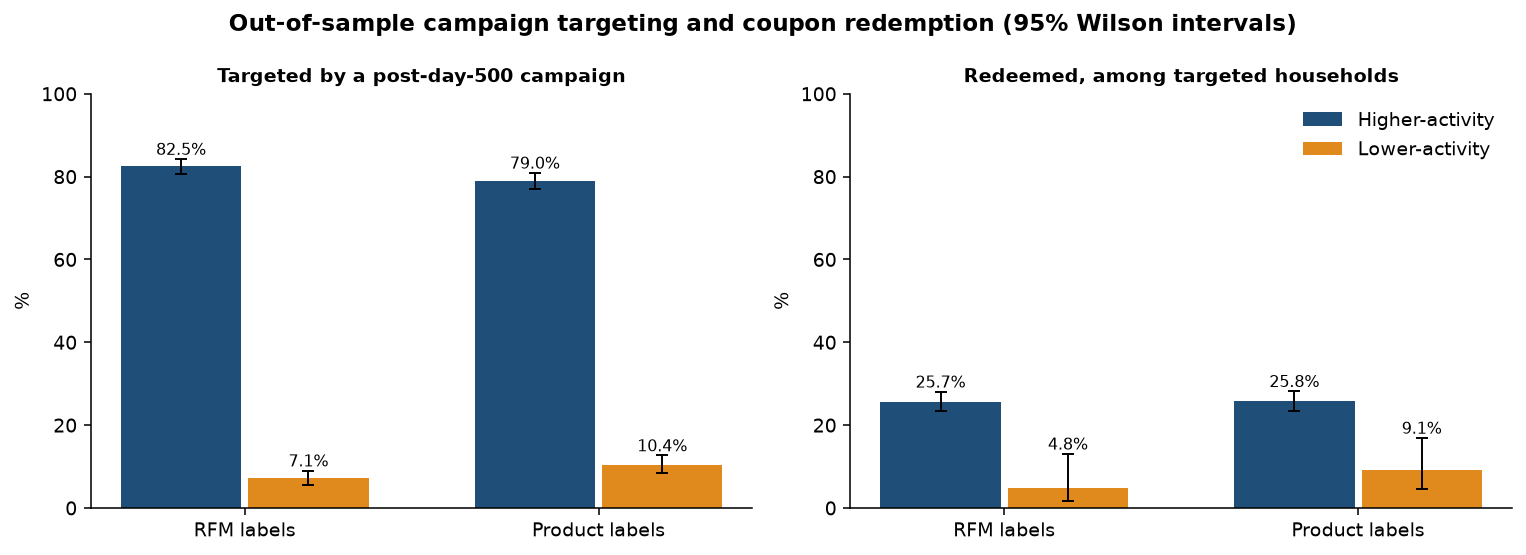
\includegraphics[width=\textwidth]{../figures/15_coupon_response.png}
\caption{Share targeted by a post-day-500 campaign and redemption rate among targeted households, with 95\% Wilson intervals.}\label{fig:coupon}
\end{figure}
Both partitions separate coupon behavior strongly. Higher-activity households are far more likely to be targeted (H$-$L gap 75.3 points for RFM, 68.6 for Product) and, once targeted, to redeem (gap 20.9 points, bootstrap CI [14.9, 26.2], $p=0.0002$ for RFM; 16.7 points, CI [9.6, 22.5], $p=0.0005$ for Product). Unconditionally, 21.2\% of RFM-H and 20.4\% of Product-H households redeem a coupon after day 500, against 0.3\% and 0.9\% in L. Product-awareness does not separate responders better: the Product-minus-RFM difference in H$-$L responder gap is $-4.2$ points with interval [$-11.8$, $+3.3$], which spans zero, and the H group's responder rate is the same in both spaces (25.7\% versus 25.8\%).

\paragraph{Limitations.} Campaign targeting was not random and is concentrated in the higher-activity group, so redemption comparisons mix household propensity with the marketer's selection; the responder rates of L households rest on 3 and 8 responders and their intervals are wide. The coupon contrast largely restates the activity gap already present in the features and cannot be read as uplift or as evidence for product-specific preferences. The demographic coverage bias above limits any claim about the low-activity group. Results describe one split of one retailer's loyalty-card sample.
